\documentclass[12pt,a4paper]{article}
\usepackage[utf8]{inputenc}
\usepackage[spanish]{babel}

\usepackage{amsmath} 
\usepackage{amsfonts}
\usepackage{amssymb}
\usepackage{graphicx}
\usepackage{ragged2e}
\usepackage{multicol}
\usepackage{multirow}
\usepackage{booktabs}
\usepackage{float}
\usepackage{enumitem}
\usepackage[left=2.54cm,right=2.54cm,top=2.54cm,bottom=2.54cm]{geometry} 
\usepackage{titlesec}
\usepackage{xurl}
\usepackage{booktabs}
\usepackage{pgfplots}
\usepackage{fontenc}
\titleformat*{\section}{\LARGE\bfseries}
\titleformat*{\subsection}{\Large\bfseries}
\titleformat*{\subsubsection}{\large\bfseries}
\titleformat*{\paragraph}{\large\bfseries}
\titleformat*{\subparagraph}{\large\bfseries}
\setcounter{topnumber}{20}
\setlength{\parindent}{0.5in}
% Useful packages
\usepackage{float}
\usepackage{amsmath}
\usepackage{graphicx}
\usepackage[colorlinks=true, allcolors=blue]{hyperref}
%%%%%%%%%%%%%%%%%%%%%%%%%%%%%%%%%%%%%%%%%%%%%%%%
%% Bibliotecas útiles %%
\usepackage{color}
\usepackage{fancyvrb}
\usepackage{listings}
\lstset{
  breaklines=true,
  postbreak=\mbox{\textcolor{red}{$\hookrightarrow$}\space},
}
% Configure bash
\lstdefinestyle{BashInputStyle}{
  language=bash,
  basicstyle=\small\sffamily,
  numbers=left,
  numberstyle=\tiny,
  numbersep=3pt,
  frame=tb,
  columns=fullflexible,
  linewidth=0.9\linewidth,
  xleftmargin=0.1\linewidth
}
%=========================================================================================================================================
\begin{document}

\thispagestyle{empty}
\begin{titlepage}
\centering
\begin{center}
\begin{tabular}{c c}

\includegraphics[width=0.25\textwidth]{img/gg.png}\hspace{5cm}&\hspace{6cm}
\includegraphics[width=0.25\textwidth]{img/proteco.png}\\
\end{tabular}
\end{center}

{\bfseries\LARGE Universidad Nacional Autónoma de México \par}
\vspace{1cm}
{\scshape\Large Facultad de Ingeniería \par}
{\scshape\Large PROTECO \par}
\vspace{1.75cm}
{\scshape\Large Generación: \par}
{\Large 45 \par}
\vfill
{\scshape\Large Proyecto final GNU/Linux: \par}
{\scshape\Large Shell 3000 \par}
\vfill
{\scshape\Large Integrantes: \par}
{\Large Aragón Martínez Mitzy Yaneth \par}
{\Large Peralta Romero José Guadalupe \par}
\vfill
{\Large Semestre 2024-1\par}
\vfill
{\Large 22 de septiembre de 2023 \par}
\end{titlepage}
%=======================================================================================
\newpage
\tableofcontents
\newpage 
%=======================================================================================
\section{Introducción}
\noindent En el presente trabajo se hace uso del Sistema Operativo GNU/Linux para la generación de una terminal en la cual un usuario pueda acceder a una serie de opciones que le permitan navegar entre las funciones permitidas, así como obtener información del sistema.

GNU/Linux es un sistema operativo open source, es decir, es un código diseñado de manera que sea accesible al público que permite a cualquiera utilizar, modificar y distribuir el sistema de forma gratuita. Este sistema operativo proporciona una plataforma estable y segura para la ejecución de programas, la gestión de archivos y la flexibilidad para adaptar el sistema a necesidades específicas del usuario, es por estos motivos que se adapta a las necesidades requeridas para el desarrollo de la terminal, principalmente porque permite la ejecución de Shell Scripts.

Así pues Shell Script es un programa que permite la creación de instrucciones que posteriormente son ejecutadas por una shell, es decir, por un intérprete de comandos. La principal función de estos programas es que, mediante la combinación de una serie de comandos y secuencias de control de flujo se puedan automatizar tareas y realizar procesos más complejos de los que un solo comando puede efectuar.

Son por estas características que para el desarrollo y ejecución de este trabajo se hace uso de Shell Script en Linux para la creación de comandos que permitan el acceso a diferentes archivos, información o actividades como lo son:

\begin{itemize}
    \item Un sistema de acceso que permita al usuario ingresar una identificación y una contraseña para el acceso a la terminal
    \item Una interfaz por medio de la cual el usuario a través de una línea de comandos pueda interactuar con el programa presentado. Los comandos disponibles podrán ejecutarse adecuadamente además de que se anularan las salidas forzadas del programa.
\end{itemize}

\noindent Por medio de esta interfaz el usuario será capaz de ingresar a los siguientes comandos:

\begin{itemize}
    \item Un comando que ofrezca ayuda al usuario al proporcionar una lista de los comandos que puede seleccionar
    \item Un comando que proporcione la información del sistema, es decir, la memoria RAM, la arquitectura del sistema y la versión del sistema operativo
    \item Un comando que proporcione la fecha y hora al usuario 
    \item Un comando que al proporcionar el nombre de un archivo y ruta en la cual está localizado pueda buscarlo y mostrar si el archivo en cuestión se encuentra en el lugar indicado.
    \item Un comando que despliegue un juego de gato, en el cual pueden interactuar dos jugadores para definir al ganador.
    \item Un comando que ofrezca una interfaz gráfica que despliegue un reproductor mp3, en el cual el usuario pueda reproducir canciones, logrando cambiar entre estas, además de observar cuál es la canción que se está reproduciendo.
    \item Un comando que muestre los créditos de los programadores que trabajaron en la creación de la terminal proporcionada
\end{itemize}

\noindent La creación de esta terminal tiene como propósito englobar y reforzar los conocimientos adquiridos por los desarrolladores al concluir con su preparación en el curso de Linux.

\newpage
\section{Desarrollo}

\subsection{Comando ayuda}
\noindent Este comando te brinda información que te da acceso a un menú de opciones a las cuales el usuario puede ingresar. Este menú despliega los nombres específicos por medio de los cuales el usuario puede llamarlos para ejecutarlos en la terminal.

\begin{figure}[H]
    \centering
    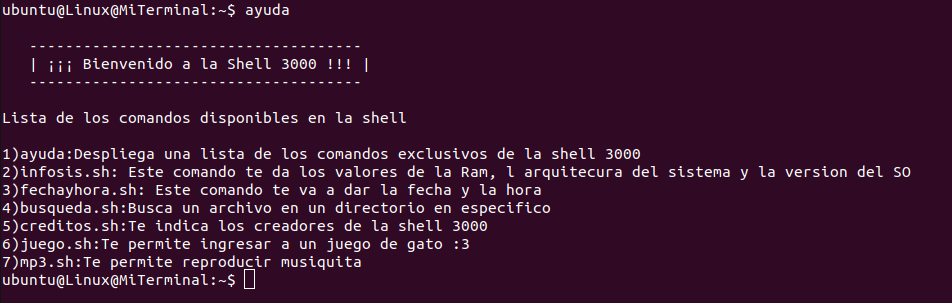
\includegraphics[width=\textwidth]{img/1.png}
    \caption{Comando ayuda}
    \label{Ayuda}
\end{figure}

\textbf{Código:}
\begin{lstlisting}[style=BashInputStyle]
echo""
echo "   -------------------------------------"
echo "   | ¡¡¡ Bienvenido a la Shell 3000 !!! |"
echo "   -------------------------------------"
echo ""
echo "Lista de los comandos disponibles en la shell"
echo ""
echo "1)ayuda:Despliega una lista de los comandos exclusivos de la shell 3000"
echo "2)infosis.sh: Este comando te da los valores de la Ram, l arquitecura del"
echo "3)fechayhora.sh: Este comando te va a dar la fecha y la hora"
echo "4)busqueda.sh:Busca un archivo en un directorio en especifico"
echo "5)creditos.sh:Te indica los creadores de la shell 3000"
echo "6)juego.sh:Te permite ingresar a un juego de gato :3"
echo "7)mp3.sh:Te permite reproducir musiquita"
\end{lstlisting}

\newpage
\subsection{Comando para juego}

\noindent Este comando te permite ingresar a una interfaz que te muestre un juego, en este caso sería el juego de gato en el cual pueden participar dos jugadores, “X” y “O”.
A modo de pantalla de inicio aparecen dos posibles opciones, jugar o no jugar gato, en caso de la primera opción se desplegará lo siguiente: 

\begin{figure}[H]
    \centering
    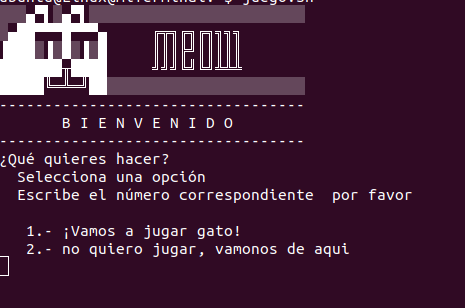
\includegraphics[width=\textwidth]{img/0.png}
    \caption{Captura de jueguito de gato miaw}
    \label{gato1}
\end{figure}

\begin{figure}[H]
    \centering
    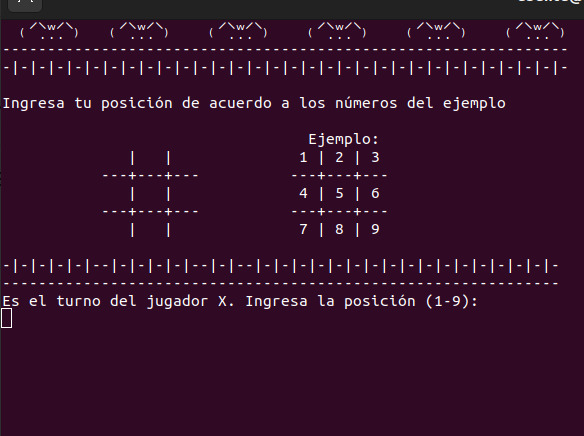
\includegraphics[width=\textwidth]{img/2.jpeg}
    \caption{Captura de jueguito de gato miaw}
    \label{gato1}
\end{figure}

\noindent Para la selección de la posición en la cual se va a localizar el jugador se escribe el número correspondiente según el ejemplo representado en el lado derecho. Los jugadores podrán seguir una partida normal de gato y una vez terminado el juego se reproduce un mensaje que indica que hay un ganador y la partida termina. En caso de que ningún jugador gane, el mensaje cambia y se muestra “empate”.

\begin{figure}[H]
    \centering
    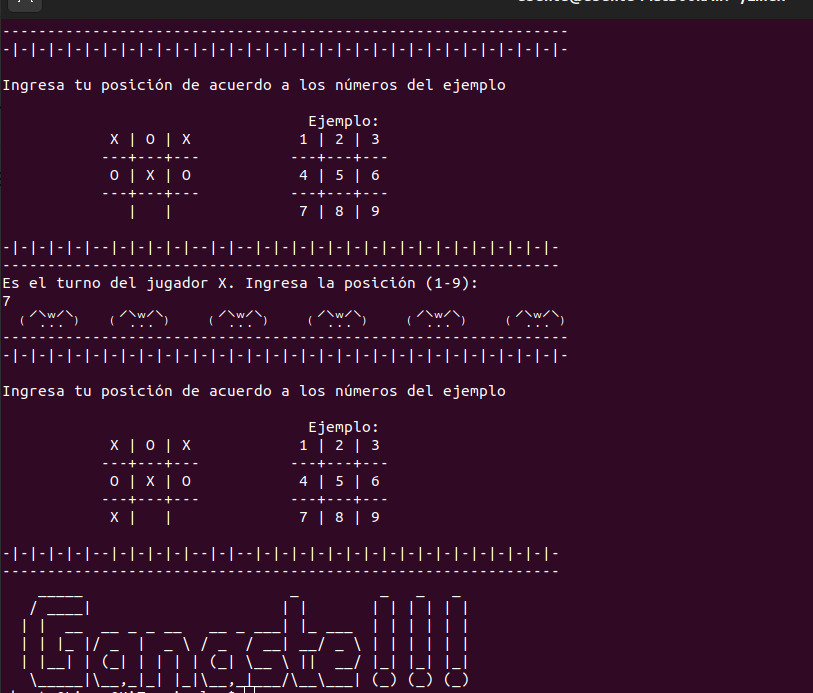
\includegraphics[width=\textwidth]{img/3.jpeg}
    \caption{Captura de jueguito de gato miaw}
    \label{gato2}
\end{figure}

\begin{figure}[H]
    \centering
    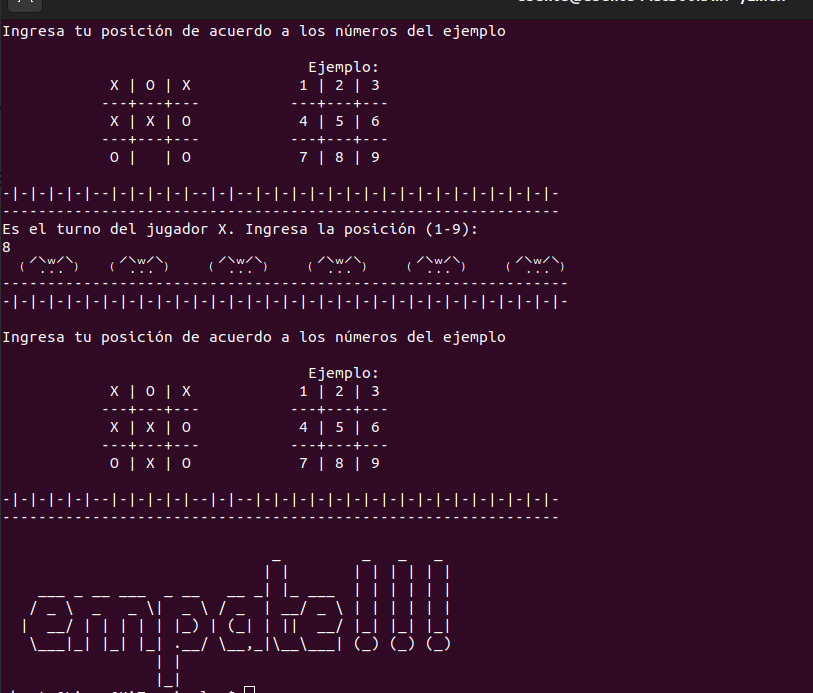
\includegraphics[width=\textwidth]{img/4.jpeg}
    \caption{Captura de jueguito de gato miaw}
    \label{gato3}
\end{figure}

\noindent En caso de que el usuario seleccione la segunda opción, es decir, no jugar se desplegará el siguiente mensaje

\begin{figure}[H]
    \centering
    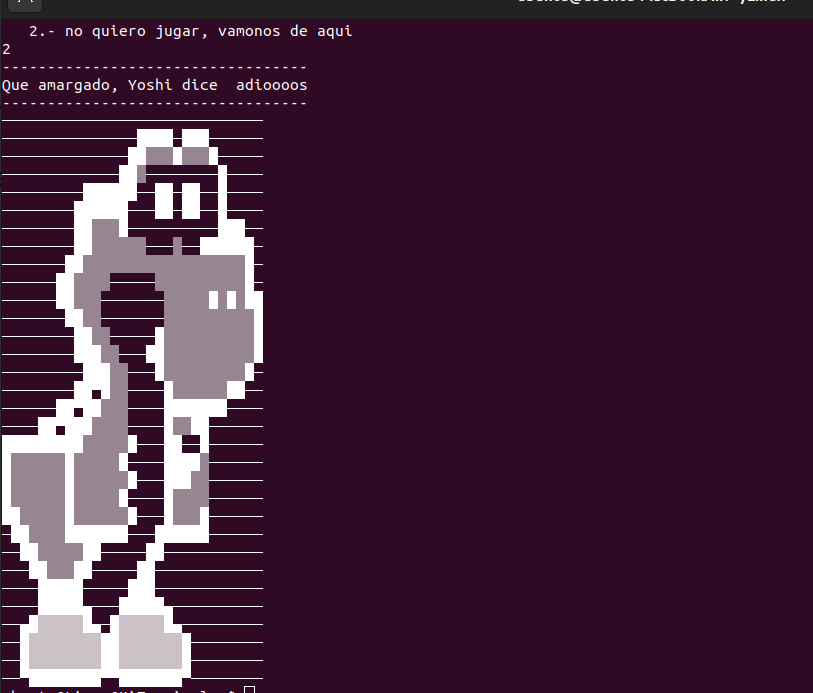
\includegraphics[width=\textwidth]{img/5.png}
    \caption{Captura de jueguito de gato miaw}
    \label{gato4}
\end{figure}
\newpage

\textbf{Código:}
\begin{lstlisting}[style=BashInputStyle]
#!/bin/bash

tablero=(" " " " " " " " " " " " " " " " " ")


mostrar_tablero() {
  
  echo "  ₍⸍⸌̣ʷ̣̫⸍̣⸌₎   ₍⸍⸌̣ʷ̣̫⸍̣⸌₎    ₍⸍⸌̣ʷ̣̫⸍̣⸌₎    ₍⸍⸌̣ʷ̣̫⸍̣⸌₎    ₍⸍⸌̣ʷ̣̫⸍̣⸌₎    ₍⸍⸌̣ʷ̣̫⸍̣⸌₎"
  echo "---------------------------------------------------------------"
  echo "-|-|-|-|-|-|-|-|-|-|-|-|-|-|-|-|-|-|-|-|-|-|-|-|-|-|-|-|-|-|-|-"
  echo ""
  echo "Ingresa tu posición de acuerdo a los números del ejemplo"
  echo ""
  echo "                                  Ejemplo:"
  echo "            ${tablero[0]} | ${tablero[1]} | ${tablero[2]}            1 | 2 | 3 "
  echo "           ---+---+---          ---+---+--- "
  echo "            ${tablero[3]} | ${tablero[4]} | ${tablero[5]}            4 | 5 | 6 "
  echo "           ---+---+---          ---+---+--- "
  echo "            ${tablero[6]} | ${tablero[7]} | ${tablero[8]}            7 | 8 | 9 "
  echo ""
  echo "-|-|-|-|-|--|-|-|-|-|--|-|--|-|-|-|-|-|-|-|-|-|-|-|-|-|-|-|-|-"
  echo "--------------------------------------------------------------"
}


verificar_ganador() {
  local ganador=""

 
  for i in 0 3 6; do
    if [[ "${tablero[$i]}" == "${tablero[$((i+1))]}" && "${tablero[$i]}" == "${tablero[$((i+2))]}" && "${tablero[$i]}" != " " ]]; then
      ganador="${tablero[$i]}"
    fi
  done

  for i in 0 1 2; do
    if [[ "${tablero[$i]}" == "${tablero[$((i+3))]}" && "${tablero[$i]}" == "${tablero[$((i+6))]}" && "${tablero[$i]}" != " " ]]; then
      ganador="${tablero[$i]}"
    fi
  done

  if [[ "${tablero[0]}" == "${tablero[4]}" && "${tablero[0]}" == "${tablero[8]}" && "${tablero[0]}" != " " ]]; then
    ganador="${tablero[0]}"
  fi

  if [[ "${tablero[2]}" == "${tablero[4]}" && "${tablero[2]}" == "${tablero[6]}" && "${tablero[2]}" != " " ]]; then
    ganador="${tablero[2]}"
  fi

  echo "$ganador"
}

jugar_gato() {
  local jugador="X"
  local empate=false
  local flag=1
  while [ $flag == 1 ]; do
    mostrar_tablero
    flag=0
    echo "Es el turno del jugador $jugador. Ingresa la posición (1-9):"
    read posicion

    if [[ ! "$posicion" =~ ^[1-9]$ ]]; then
      echo "Por favor ingresa un número aceptable del 1 al 9"
      continue
    fi

    local indice=$((posicion - 1))

    if [[ "${tablero[$indice]}" == " " ]]; then
      tablero[$indice]=$jugador
    else
      echo "Posición ya utilizada, por favor ingresa otra :3"
      flag=1
      continue
    fi

    ganador=$(verificar_ganador)

    for i in $(seq 0 8); do
      if [[ "${tablero[$i]}" == " " ]]; then
        flag=1
      fi
    done

    if [[ "$ganador" == "X" || "$ganador" == "O" ]]; then
      mostrar_tablero

	echo "    _____                       _         _   _   _ "
	echo "   / ____|                     | |       | | | | | |"
	echo "  | |  __  __ _ _ __   __ _ ___| |_ ___  | | | | | |"
	echo "  | | |_ |/ _  |  _ \ / _  / __| __/ _ \ | | | | | |"
	echo "  | |__| | (_| | | | | (_| \__ \ ||  __/ |_| |_| |_|"
	echo "   \_____|\__,_|_| |_|\__,_|___/\__\___| (_) (_) (_)"
      break
    elif [[ $flag == 0 ]]; then
      mostrar_tablero
      echo ""
	echo "                              _         _   _   _ "
	echo "                             | |       | | | | | |"
	echo "    ___ _ __ ___  _ __   __ _| |_ ___  | | | | | |"
	echo "   / _ \  _   _ \|  _ \ / _  | __/ _ \ | | | | | |"
	echo "  |  __/ | | | | | |_) | (_| | ||  __/ |_| |_| |_|"
	echo "   \___|_| |_| |_| .__/ \__,_|\__\___| (_) (_) (_)"
	echo "                 | |                              "
	echo "                 |_|                              "
      break
    fi

 
    if [[ "$jugador" == "X" ]]; then
      jugador="O"
    else
      jugador="X"
    fi
  done
}


menu_principal(){
opcion=0
echo "░░░▄▀▌░▄▀▌░░░░░░░░░░░░░░░░░░░░░░░░"
echo "░▄██▀▀▀█▀▀▀▄     ╔╦╗╔╗╔╗╗╗╗       "
echo "▐███░▐░█░▐░█     ║║║╠╝║║║║║       "
echo "███████╥████     ╝╝╝╚╝╚╝╩╩╩       "
echo "█████╚═╩═╝██░░░░░░░░░░░░░░░░░░░░░░"
echo "----------------------------------"
echo "       B I E N V E N I D O        "
echo "----------------------------------"
echo "¿Qué quieres hacer? "
echo "  Selecciona una opción "
echo "  Escribe el número correspondiente  por favor"
echo ""
echo "   1.- ¡Vamos a jugar gato!"
echo "   2.- no quiero jugar, vamonos de aqui"
read opcion
case $opcion in
1)
	clear
	jugar_gato
	;;
2)
	echo "----------------------------------"
	echo "Que amargado, Yoshi dice  adioooos"
	echo "----------------------------------"
echo  "─────────────────────────────"
echo "───────────────████─███──────"
echo "──────────────██▒▒▒█▒▒▒█─────"
echo "─────────────██▒────────█────"
echo "─────────██████──██─██──█────"
echo "────────██████───██─██──█────"
echo "────────██▒▒▒█──────────███──"
echo "────────██▒▒▒▒▒▒───▒──██████─"
echo "───────██▒▒▒▒▒▒▒▒▒▒▒▒▒▒▒▒▒▒█─"
echo "──────██▒▒▒▒─────▒▒▒▒▒▒▒▒▒▒█─"
echo "──────██▒▒▒───────▒▒▒▒▒█▒█▒██"
echo "───────██▒▒───────▒▒▒▒▒▒▒▒▒▒█"
echo "────────██▒▒─────█▒▒▒▒▒▒▒▒▒▒█"
echo "────────███▒▒───██▒▒▒▒▒▒▒▒▒▒█"
echo "─────────███▒▒───█▒▒▒▒▒▒▒▒▒█─"
echo "────────██▀█▒▒────█▒▒▒▒▒▒██──"
echo "──────██▀██▒▒▒────███████────"
echo "────██▀███▒▒▒▒────█▒▒██──────"
echo "█████████▒▒▒▒▒█───██──█──────"
echo "█▒▒▒▒▒▒█▒▒▒▒▒█────████▒──────"
echo "█▒▒▒▒▒▒█▒▒▒▒▒▒█───███▒▒──────"
echo "█▒▒▒▒▒▒█▒▒▒▒▒█────█▒▒▒▒──────"
echo "██▒▒▒▒▒█▒▒▒▒▒▒█───█▒▒▒█──────"
echo "─██▒▒▒▒███████───██████──────"
echo "──██▒▒▒▒▒██─────██───────────"
echo "───██▒▒▒██─────██────────────"
echo "────█████─────███────────────"
echo "────█████▄───█████▄──────────"
echo "──▄█▓▓▓▓▓█▄─█▓▓▓▓▓█▄─────────"
echo "──█▓▓▓▓▓▓▓▓██▓▓▓▓▓▓▓█────────"
echo "──█▓▓▓▓▓▓▓▓██▓▓▓▓▓▓▓█────────"
echo "──▀████████▀▀███████▀────────"

	exit
	;;
*)
	echo "esa no es una opción valida"
	;;
esac

}

menu_principal
\end{lstlisting}

\newpage
\subsection{Comando infosis}

\noindent En este comando el usuario puede acceder a la información del sistema en el que se encuentra, tal información está conformada por la memoria RAM, la arquitectura del sistema y la versión del sistema operativo. Para obtener esta información de la RAM se accede a la carpeta “meminfo” de la cual se extrae la información de MemTotal; para obtener la arquitectura del sistema se accede a la carpeta version en donde se busca y accede a  “model name”; para obtener la versión del sistema operativo se accede a la carpeta de os-release en la cual se busca y extrae la información de “PRETTY\_NAME”. Posteriormente estas informaciones extraídas se guardan en variables que se muestran al usuario.

\begin{figure}[H]
    \centering
    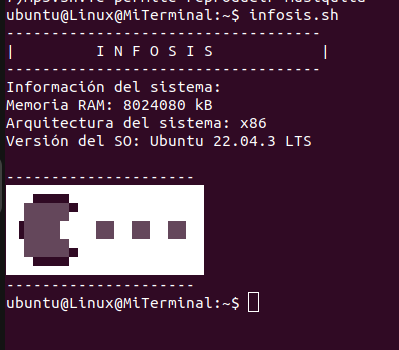
\includegraphics[width=\textwidth]{img/infosis.png}
    \caption{Captura de comando infosis}
    \label{infosis}
\end{figure}

\newpage
\textbf{Código:}
\begin{lstlisting}[style=BashInputStyle]
  GNU nano 6.2                                                          infosis.sh                                                                    
# Arquitectura del Sistema desde /proc/version
arquitectura=$(grep 'model name' /proc/cpuinfo | head -n 1 | awk '{print $4}')
if [[ "$arquitectura" == "lm" ]]; then
  arquitectura="x86_64"
else
  arquitectura="x86"
fi
# Versión del SO desde /etc/os-release
version_so=$(grep 'PRETTY_NAME' /etc/os-release | awk -F '=' '{print $2}' | tr -d '"')


echo "-----------------------------------"
echo "|         I N F O S I S            |"
echo "-----------------------------------"

echo "Información del sistema:"
echo "Memoria RAM: $memoria_ram kB"
echo "Arquitectura del sistema: $arquitectura"
echo "Versión del SO: $version_so"


echo ""
echo "---------------------"
echo "███▀▀▀▀███████████████"
echo "██░░░░░▄██████████████"
echo "█▌░░░░████░░██░░██░░██"
echo "██░░░░░▀██████████████"
echo "███▄▄▄▄███████████████"
echo "---------------------"
\end{lstlisting}

\newpage
\subsection{Comando fecha y hora}
\noindent Este comando permite al usuario acceder a la información del sistema de fecha y hora. Para lograr esto se ingresa a la carpeta de rtc la cual gestiona el reloj en tiempo real. 
Usar la carpeta del componente RTC es una buena opción ya que este hardware mantiene un seguimiento del tiempo aun cuando la computadora está apagada o reiniciada. Una vez en la carpeta rtc se extrae la información de  “rtc\_time” y “rtc\_date”, proporcionando así la  hora en formato hora, minuto, segundos y la fecha en formato año, mes y día.

\begin{figure}[H]
    \centering
    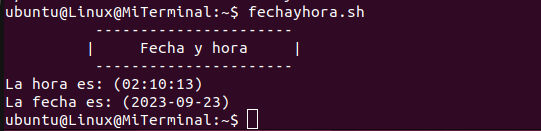
\includegraphics[width=\textwidth]{img/fyh.png}
    \caption{Captura de comando de fecha y hora}
    \label{fyh}
\end{figure}

\textbf{Código:}
\begin{lstlisting}[style=BashInputStyle]
#!/bin/bash

echo "          ----------------------"
echo "         |     Fecha y hora     |"
echo "          ----------------------"



hora=$(cat /proc/driver/rtc | grep "rtc_time" | sed 's/rtc_time[ \t]*:[ \t]*//')
echo "La hora es: ($hora)"

fecha=$(cat /proc/driver/rtc| grep "rtc_date"| sed 's/rtc_date[ \t]*:[ \t]*//')

echo "La fecha es: ($fecha)"
echo ":3"
\end{lstlisting}

\newpage
\subsection{Comando para la búsqueda de archivos}
\noindent Este comando permite la búsqueda de un archivo para lo cual la shell recibe la ruta absoluta ingresada por el usuario así como el nombre del archivo que quiere localizar, posteriormente con “-e” procede a realizar la búsqueda y finalmente si la encuentra proyecta un mensaje informando que encontró lo solicitado, en caso contrario cambia el mensaje indicando que no se encuentra en la dirección proporcionada.

\begin{figure}[H]
    \centering
    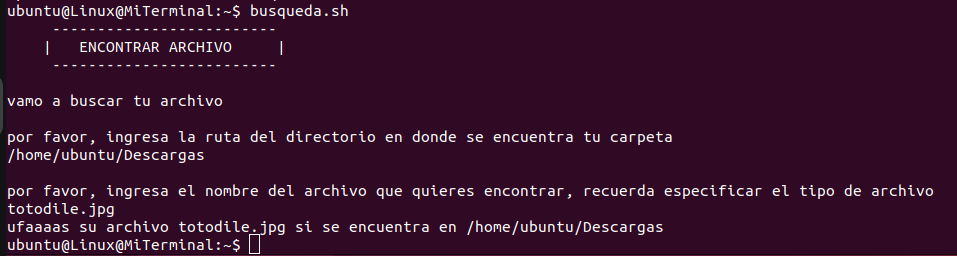
\includegraphics[width=\textwidth]{img/a1.png}
    \caption{Captura de comando para búsqueda de archivos}
    \label{arch1}
\end{figure}

\begin{figure}[H]
    \centering
    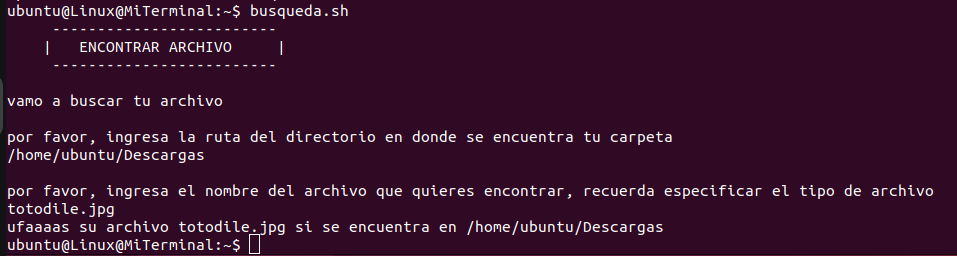
\includegraphics[width=\textwidth]{img/a2.png}
    \caption{Captura de comando para búsqueda de archivos}
    \label{arch2}
\end{figure}

\newpage
\textbf{Código:}
\begin{lstlisting}[style=BashInputStyle]
#!/bin/bash

# Un comando que pueda buscar por un archivo en un directorio específico recibe
#dos  parámetros: La carpeta a buscar y el archivo que va a buscar.
#Ej: Linux GEN 44

echo "     -------------------------"
echo "    |   ENCONTRAR ARCHIVO     | "
echo "     -------------------------"
echo ""
echo "vamo a buscar tu archivo"
echo ""
echo "por favor, ingresa la ruta absoluta del directorio en donde se encuentra tu carpeta"
read  rutaCarpeta
echo ""
echo "por favor, ingresa el nombre del archivo que quieres encontrar, recuerda especificar el tipo de archivo"
read nombreArchivo

#rutaCarpeta="$(realpath "$rutaCarpeta")"
rutaCarpeta_y_nombreArchivo="$rutaCarpeta/$nombreArchivo"

if [ -e "$rutaCarpeta_y_nombreArchivo" ]; then
	echo "ufaaaas su archivo $nombreArchivo si se encuentra en $rutaCarpeta"
else
	echo "nooo puede ser su archivo $nombreArchivo no se ha encontrado en $rutaCarpeta, que triste tu caso"

fi
\end{lstlisting}

\newpage
\subsection{Comando para los créditos}
\noindent Este comando muestra con una función simple de echo los créditos de los programadores que se rifaron semejante proyecto, más chulo de hermoso realizado con todo su corazón, sudor, ansiedad, lágrimas y pocos conocimientos al no ser de cómputo. Tal vez es poco pero es un trabajo honesto. 

\begin{figure}[H]
    \centering
    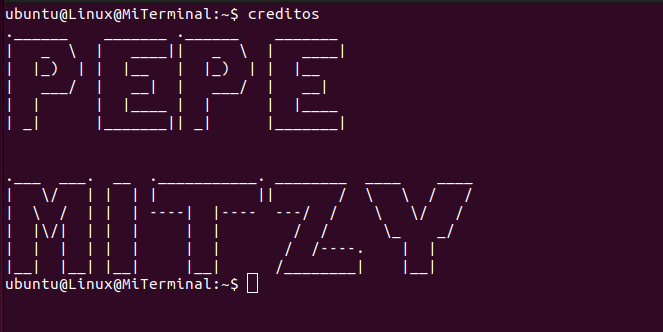
\includegraphics[width=\textwidth]{img/cr.png}
    \caption{Captura de comando para mostrar los créditos}
    \label{creditos}
\end{figure}

\textbf{Código:}
\begin{lstlisting}[style=BashInputStyle]
echo ".______    _______ .______    _______     "
echo "|   _  \  |   ____||   _  \  |   ____|    "
echo "|  |_)  | |  |__   |  |_)  | |  |__       "
echo "|   ___/  |   __|  |   ___/  |   __|      "
echo "|  |      |  |____ |  |      |  |____    "
echo "| _|      |_______|| _|      |_______|   "
echo ""
echo ""

echo ".___  ___.  __  .___________. ________  ____    ____     "
echo "|   \/   | |  | |           ||       /  \   \  /   /     "
echo "|  \  /  | |  | ----|  |----  ---/  /    \   \/   /      "
echo "|  |\/|  | |  |     |  |        /  /      \_    _/       "
echo "|  |  |  | |  |     |  |       /  /----.    |  |         "
echo "|__|  |__| |__|     |__|      /________|    |__|         "
\end{lstlisting}

\newpage
\subsection{Comando para reproductor mp3}
\noindent Al ingresar a este comando al usuario se le desplegarán dos menús, el primero da información de las opciones que tiene de reproducción de música, de las canciones que puede reproducir así como de la opción de salida.
En el segundo menú se muestran las opciones que puede escoger el usuario para mejorar y adaptar su experiencia al reproducir la música, es decir, pausar la canción , reproducir la siguiente o anterior rola, subir o bajar volumen, regresar la canción al principio y salir del reproductor.
Posteriormente una vez el usuario lee las opciones puede ingresar las opciones que eligió para que la musiquita empiece a sonar y diga subele a la radio.
Este comando se basa en la creación de una  segunda terminal en la cual se redimensiona al usuario a la ruta seleccionada para el acceso a las canciones disponibles..


\begin{figure}[H]
    \centering
    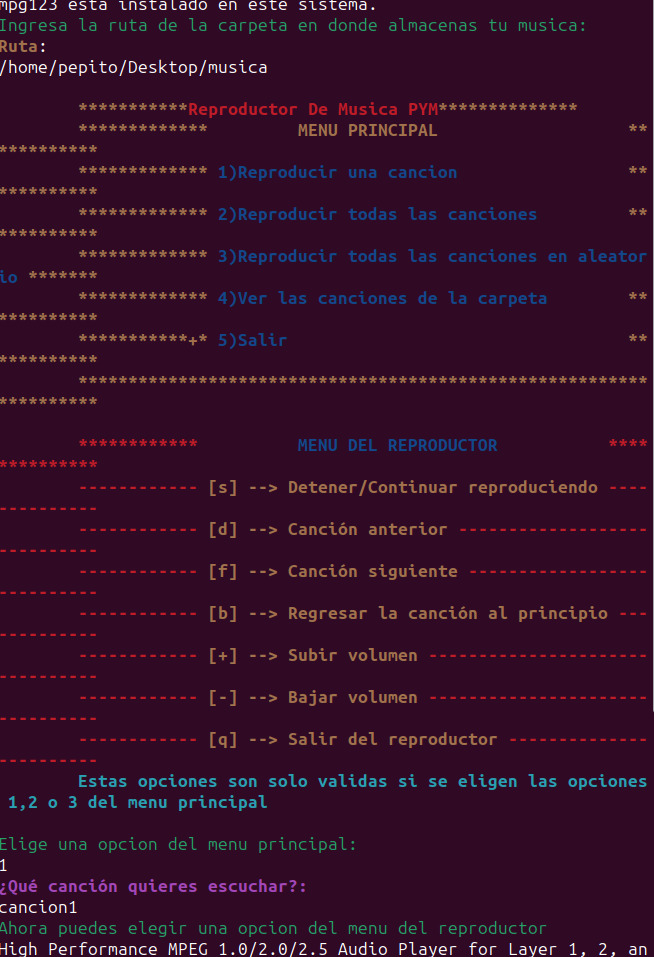
\includegraphics[width=0.95\textwidth]{img/mp3.jpeg}
    \caption{Captura de comando para reproduccion de mp3}
    \label{mp3}
\end{figure}

\newpage
\textbf{Código:}
\begin{lstlisting}[style=BashInputStyle]
# Verifica si mpg123 está instalado
	if command -v mpg123 &>/dev/null; then
	    echo "mpg123 está instalado en este sistema."
	else
	    echo "mpg123 no está instalado en este sistema.Porfavor utilice en su terminal sudo apt-install mpg123 si desea utilizar este super reproductor"
	    exit
	fi
	
	
	


	
	control=0
	#Ruta de la carpeta en donde se encuentra la musica
	echo -e  "\e[0;32mIngresa la ruta de la carpeta en donde almacenas tu musica:\e[0m "
	echo -e "\e[1;33mRuta\e[0m: "
	read ruta
	cd $ruta


	#Empieza el ciclo para mostrar el menu y hacer las operaciones de la prebeplayer
	while [ $control -ne 1 ];
	do
		#Menu de la prebeplayer
		echo -e "\n\t\e[1;33m***********\e[0m\e[1;31mReproductor De Musica PYM\e[0m\e[1;33m**************\e[0m"
		echo -e "\t\e[1;33m*************\e[0m         \e[1;33mMENU PRINCIPAL\e[0m                   \e[1;33m************\e[0m"
		echo -e "\t\e[1;33m*************\e[0m \e[1;34m1)Reproducir una cancion\e[0m                 \e[1;33m************\e[0m"
		echo -e "\t\e[1;33m*************\e[0m \e[1;34m2)Reproducir todas las canciones\e[0m         \e[1;33m************\e[0m"
		echo -e "\t\e[1;33m*************\e[0m \e[1;34m3)Reproducir todas las canciones en aleatorio\e[0m \e[1;33m*******\e[0m"
		echo -e "\t\e[1;33m*************\e[0m \e[1;34m4)Ver las canciones de la carpeta\e[0m        \e[1;33m************\e[0m"
		echo -e "\t\e[1;33m***********+*\e[0m \e[1;34m5)Salir\e[0m                                  \e[1;33m************\e[0m"
		echo -e "\t\e[1;33m*******************************************************************\e[0m"
		echo -e "\n\t\e[1;31m************\e[0m          \e[1;34mMENU DEL REPRODUCTOR\e[0m           \e[1;31m**************\e[0m"
                echo -e "\t\e[1;31m------------\e[0m \e[1;33m[s] --> Detener/Continuar reproduciendo\e[0m \e[1;31m--------------\e[0m"
                echo -e "\t\e[1;31m------------\e[0m \e[1;33m[d] --> Canción anterior\e[0m \e[1;31m-----------------------------\e[0m"
                echo -e "\t\e[1;31m------------\e[0m \e[1;33m[f] --> Canción siguiente\e[0m \e[1;31m----------------------------\e[0m"
                echo -e "\t\e[1;31m------------\e[0m \e[1;33m[b] --> Regresar la canción al principio\e[0m \e[1;31m-------------\e[0m"
                echo -e "\t\e[1;31m------------\e[0m \e[1;33m[+] --> Subir volumen\e[0m \e[1;31m--------------------------------\e[0m"
                echo -e "\t\e[1;31m------------\e[0m \e[1;33m[-] --> Bajar volumen\e[0m \e[1;31m--------------------------------\e[0m"
                echo -e "\t\e[1;31m------------\e[0m \e[1;33m[q] --> Salir del reproductor\e[0m \e[1;31m------------------------\e[0m"
                echo -e "\t\e[1;36mEstas opciones son solo validas si se eligen las opciones 1,2 o 3 del menu principal\e[0m"

		#Solicita la eleccion de una opcion del menu que se le va a mostar
		echo -e "\n\e[0;32mElige una opcion del menu principal: \e[0m"
		read opcion
		#Control de las acciones para cada opcion del menu
		case $opcion in
			1)
				#Le permite al usuario elegir la cancion que va a escuchar
				echo -e "\e[1;35m¿Qué canción quieres escuchar?: \e[0m"
				read cancion
				echo -e  "\e[0;32mAhora puedes elegir una opcion del menu del reproductor\e[0m"
				#Comando que se encarga de reproducir la canción que se le indica en formato mp3
				mpg123 -C /$ruta/"$cancion.mp3"
				

			;;

			2)
				#Reproduce todas las canciones dentro de la carpeta de musica que el  usuario indico
				echo -e "\e[1;35mVamos a armar un pachangon con tu playlist\e[0m"
				echo -e  "\e[0;32mAhora puedes elegir una opcion del menu del reproductor\e[0m"
				#Comando para reproducir todas las canciones
				mpg123 -C /$ruta/*
                        ;;


			3)
				#Reproduce todas las canciones dentro de la carpeta de musica que el usuario le indico
				echo -e "\e[1;35mVamos a armar un pachangon aleatorio con tu playlist\e[0m"
				echo -e  "\e[0;32mAhora puedes elegir una opcion del menu del reproductor\e[0m"
				#Comando para reproducir en modo aleatorio
				mpg123 -C -z /$ruta/*
                        ;;

			4)
				echo "Las canciones son:"
				ls $ruta
			;;


			5)
				control=1
			;;

			*)
				#Indica que hubo error si el usuario bobo no eligió algo del menu
				echo -e  "\e[1;35mOpción no válida, intentalo de nuevo plis\e[0m"
			;;


		esac
	done
\end{lstlisting}

\newpage
\section{Conclusiones}

\begin{itemize}
    \item \textbf{Aragón Martínez Mitzy Yaneth:}  La realización de este proyecto de una terminal en Linux ha sido un ejercicio valioso que ha proporcionado una comprensión más profunda de este sistema operativo y de cómo interactuamos con él a través de línea de comandos. A lo largo de este proyecto, pudimos mejorar nuestras habilidades de programación, especialmente en Shell Script, así como en la manipulación de archivos, la gestión de procesos, la interpretación de comandos, la gestión de recursos y de segurdad y permisos. Por último, pero no menos importante, desarrollamos nuestra capacidad de trabajo en equipo, organización, y comunicación, dado que trabajamos en conjunto y además utilizamos las herramientas de Git y Github para el manejo del control de versiones.
    
    \item \textbf{Peralta Romero José Guadalupe:} La ejecución de este proyecto de crear una terminal simulada en el entorno Linux se ha revelado como una experiencia extremadamente beneficiosa que nos ha brindado una comprensión más profunda de cómo opera este sistema operativo y de nuestra interacción con él a través de la línea de comandos. Durante el desarrollo de este proyecto, no solo tuvimos la oportunidad de perfeccionar nuestras habilidades de programación, centrándonos en Shell Script, sino que también adquirimos un dominio más sólido en áreas esenciales como la manipulación de archivos, la administración de procesos, la interpretación de comandos, la gestión de recursos y la implementación de medidas de seguridad y permisos. No obstante, el valor de este proyecto trascendió la mera mejora de habilidades técnicas. Se convirtió en una experiencia de desarrollo personal y de equipo. Trabajar juntos en la creación de esta terminal simulada nos permitió fortalecer nuestras habilidades de trabajo en equipo, organización y comunicación. Fue un terreno fértil para la colaboración, donde aprendimos a enfrentar desafíos técnicos y a resolver problemas de manera conjunta. Además, no podemos pasar por alto la introducción al mundo de Git y Github. Utilizar estas herramientas para el control de versiones fue un paso importante en nuestro proceso de aprendizaje y colaboración. Nos enseñó cómo llevar un seguimiento eficiente de nuestros cambios, mantener la coherencia en el proyecto y facilitar la contribución de cada miembro del equipo. En resumen, este proyecto no solo nos brindó conocimientos técnicos valiosos, sino que también enriqueció nuestras habilidades de colaboración y gestión de proyectos. Nos prepara para abordar futuros desafíos en el vasto campo de la informática con confianza y competencia.
\end{itemize}

\newpage
% \bibliographystyle{apalike2-espa}
% \bibliography{refs.bib}
\end{document}
